\documentclass[11pt]{article}

\usepackage{graphicx}

\graphicspath{ {.} }

% Margins
\topmargin=-0.45in
\evensidemargin=0in
\oddsidemargin=0in
\textwidth=6.5in
\textheight=9.0in
\headsep=0.25in

\title{ Analysis of Classification models}
\author{Arnav Rustagi}
\date{\today}

\begin{document}
\maketitle	

\section {Q3 : metrics of the LSTM}
url : https://github.com/thearnavrustagi/sentiment\_classifier.git\\
epochs : 15
\begin{center}
	\begin{tabular}{ |c|c|c|c| } 
 \hline
	accuracy (eval) & loss (eval) & accuracy (train) & loss (train) \\ 
 \hline
	 66.40625 \% & 2.4213303327560425 & 95.12018\% &  0.02476043999195099 \\ 
 \hline
\end{tabular}
\end{center}
confusion matrix :
\begin {center}
	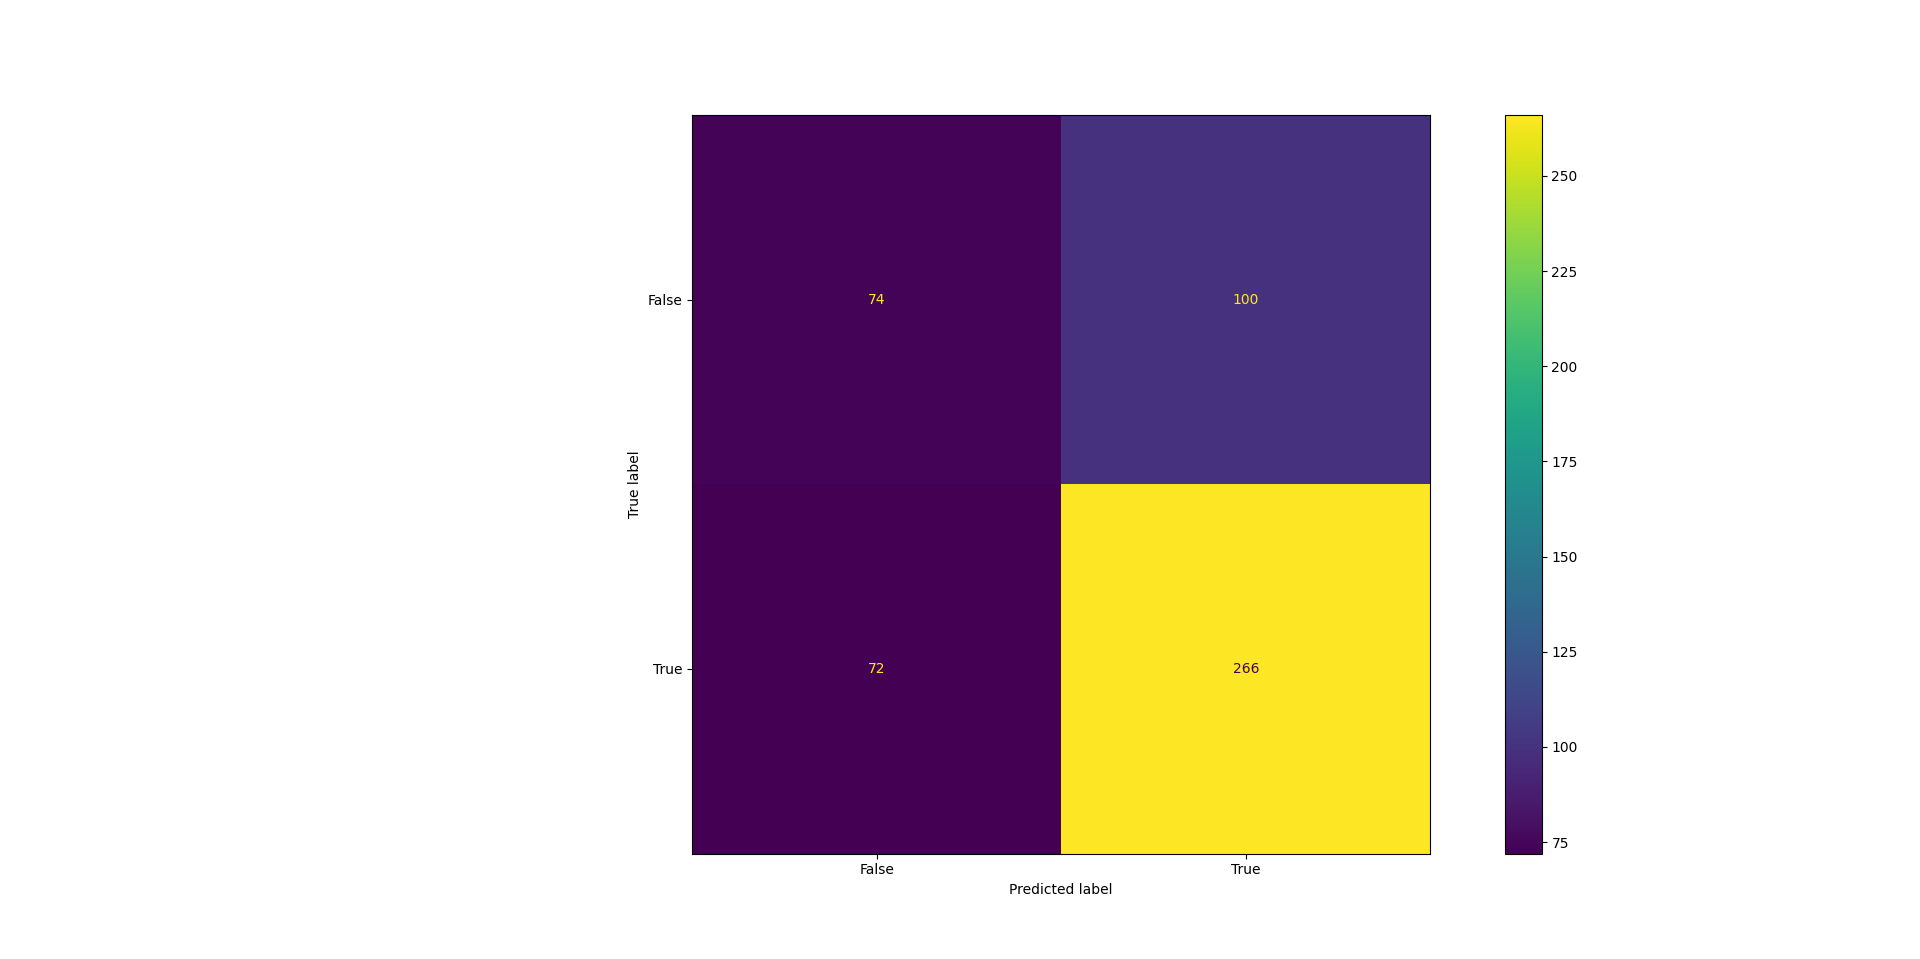
\includegraphics[width=\textwidth]{lstm_cm}
\end {center}
\section {Q4 : metrics of the BERT with Sequence Classification head}
url : https://colab.research.google.com/drive/1tn4i77WhzP2jHUjq4ES-zvNk9W3SAelt?usp=sharing\\
epochs : 15
\begin{center}
\begin{tabular}{ |c|c|c|c| } 
 \hline
	accuracy (eval) & loss (eval) & accuracy (train) & loss (train) \\ 
 \hline
	 82.14 \% & 0.7539991132696287 & 84.0027\% &  0.023000 \\ 
 \hline
\end{tabular}
\end{center}
\begin {center}
	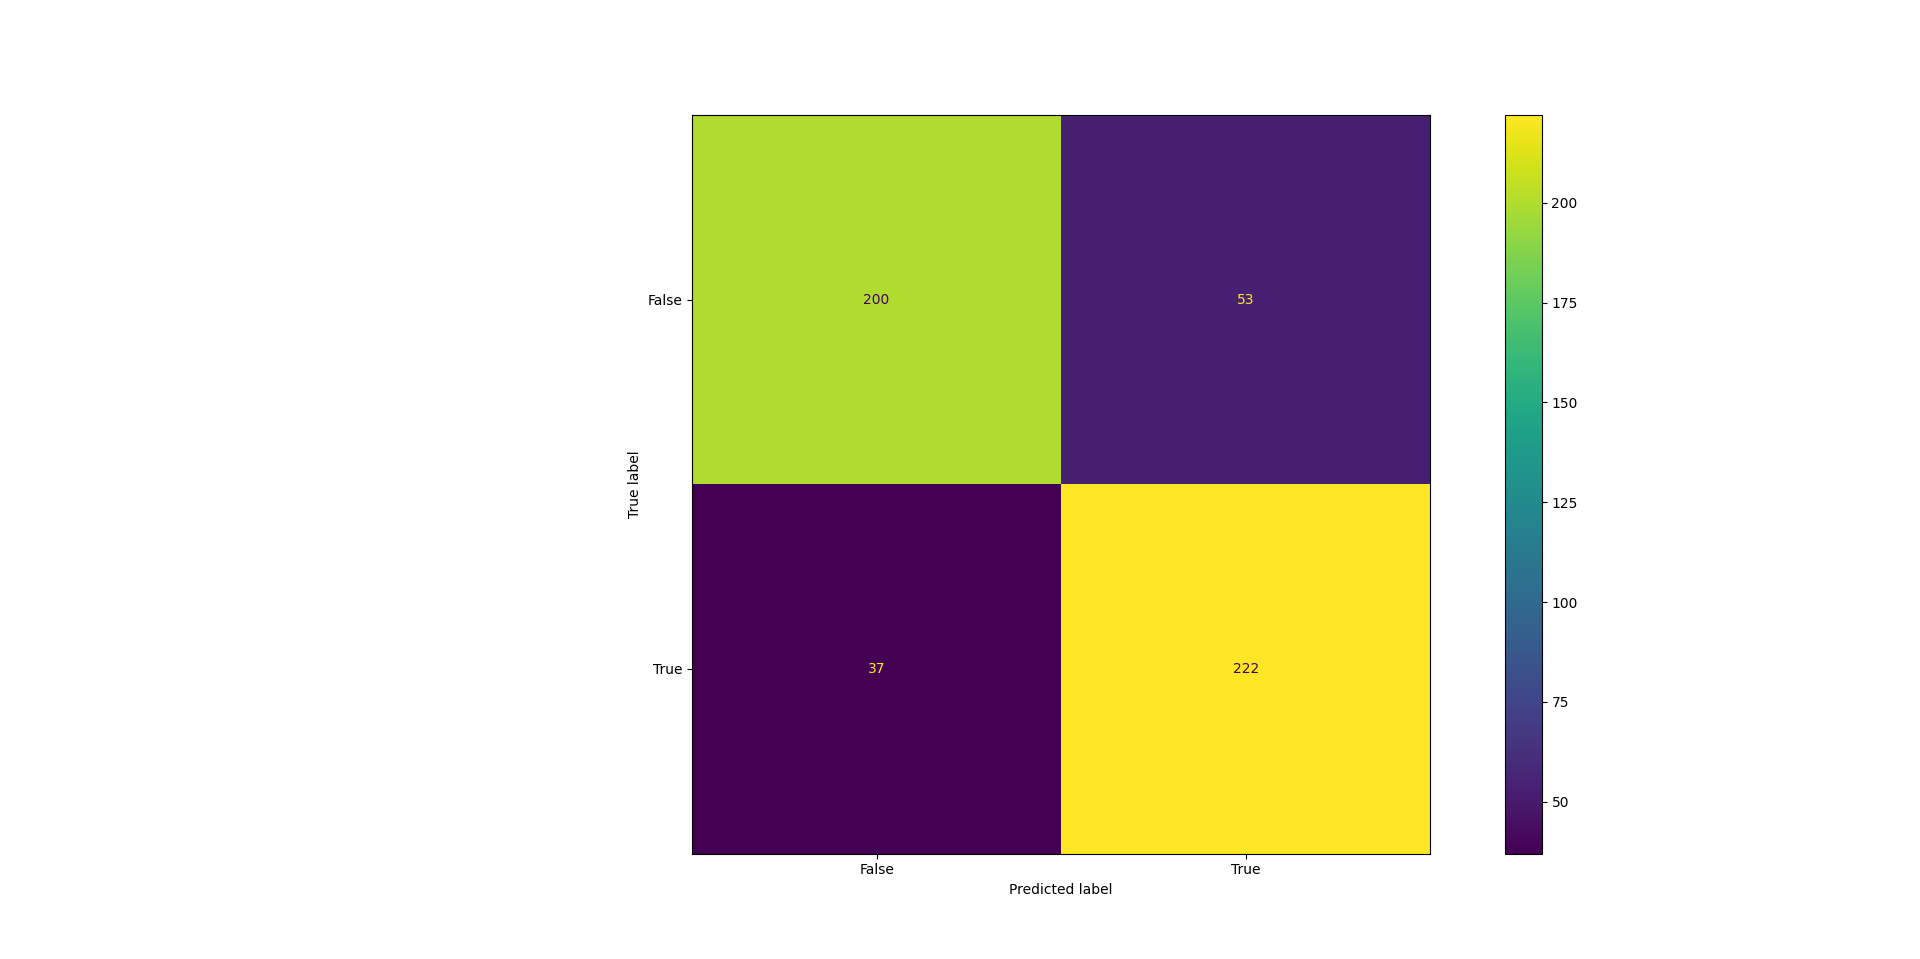
\includegraphics[width=\textwidth]{bert_cm}
\end {center}
\section {Q5 : analysis}
As you can see on the metrics, eventhough both the models had the same loss during training, it is quite evident that the loss during evaluation was much higher for the LSTM, this might have been due to overfitting which can also be seen in the accuracy. The accuracy of the BERT is similar in training and validation, but for the LSTM it is much higher for training than for validation, as it has evidently overfitted the dataset.
\\\\
Moreover as LSTM is recurrent network and can not see every token, it is inferior to BERT which can look at each token while creating the encoded representation.
\\\\
Though I would conclude that the LSTM is overfit and thats the reason for such a discrepency in accuracy and loss, which is not the case for the BERT. Another problem with the LSTM that I concluded was the lack of Byte-Pair Encoding, and using word based encoding which might have caused many words to be replaced with the $<UNK>$ token, as the validation data was from indian origin, and had words like "modi" which the LSTM would have been unable to truly understand.
\\\\
Maybe to prevent overfitting when retraining the model we can use sentence transformers to create some noise in the data. Moreover the lack of layer normalization also might have affected not only the training quality but also aided overfitting. another thing we can test is increasing the dropout, but increasing dropout from $0.15$ might be too much.
\end{document}
